% Created by tikzDevice version 0.10.1 on 2017-10-30 17:28:49
% !TEX encoding = UTF-8 Unicode
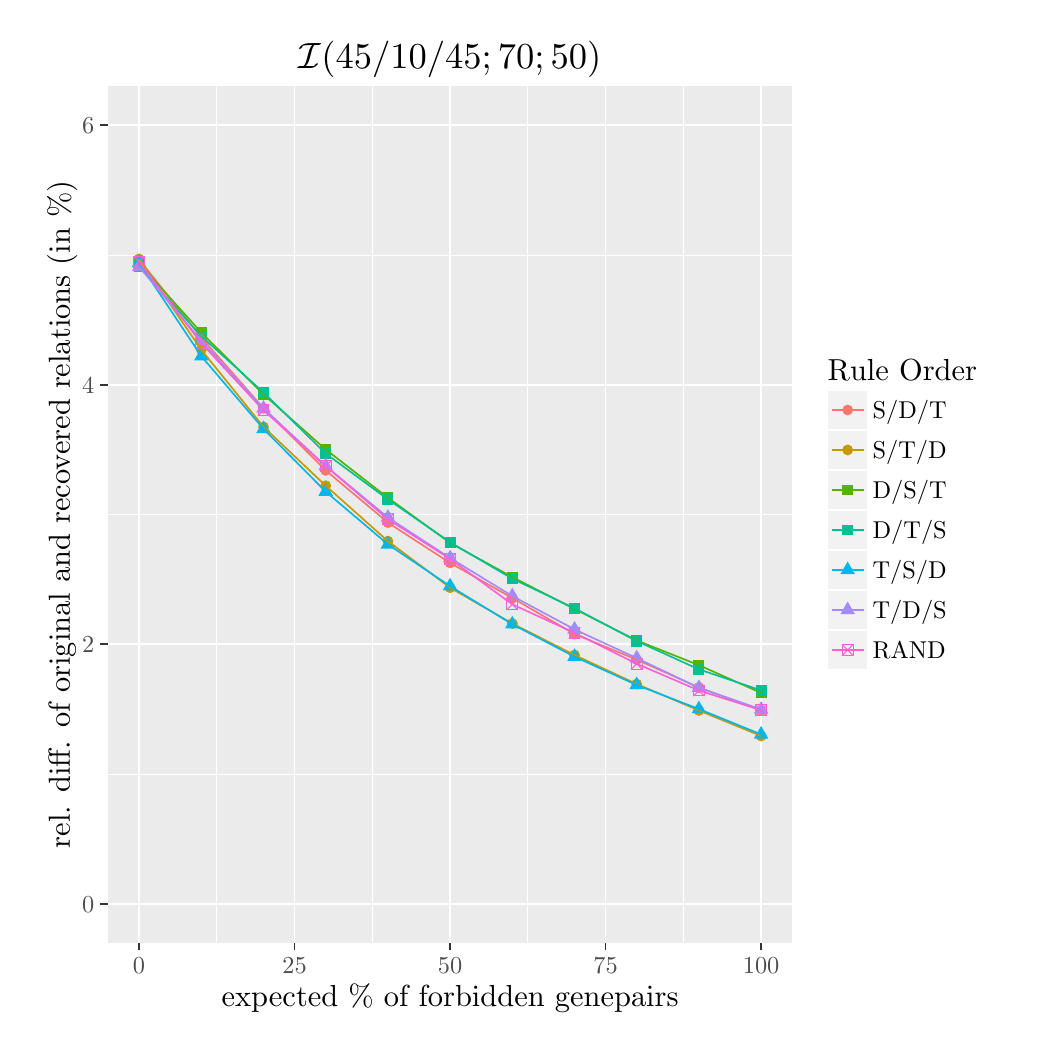
\begin{tikzpicture}[x=1pt,y=1pt]
\definecolor{fillColor}{RGB}{255,255,255}
\path[use as bounding box,fill=fillColor,fill opacity=0.00] (0,0) rectangle (361.35,361.35);
\begin{scope}
\path[clip] (  0.00,  0.00) rectangle (361.35,361.35);
\definecolor{drawColor}{RGB}{255,255,255}
\definecolor{fillColor}{RGB}{255,255,255}

\path[draw=drawColor,line width= 0.6pt,line join=round,line cap=round,fill=fillColor] (  0.00,  0.00) rectangle (361.35,361.35);
\end{scope}
\begin{scope}
\path[clip] ( 29.02, 30.69) rectangle (276.26,340.16);
\definecolor{fillColor}{gray}{0.92}

\path[fill=fillColor] ( 29.02, 30.69) rectangle (276.26,340.16);
\definecolor{drawColor}{RGB}{255,255,255}

\path[draw=drawColor,line width= 0.3pt,line join=round] ( 29.02, 91.64) --
	(276.26, 91.64);

\path[draw=drawColor,line width= 0.3pt,line join=round] ( 29.02,185.42) --
	(276.26,185.42);

\path[draw=drawColor,line width= 0.3pt,line join=round] ( 29.02,279.20) --
	(276.26,279.20);

\path[draw=drawColor,line width= 0.3pt,line join=round] ( 68.36, 30.69) --
	( 68.36,340.16);

\path[draw=drawColor,line width= 0.3pt,line join=round] (124.55, 30.69) --
	(124.55,340.16);

\path[draw=drawColor,line width= 0.3pt,line join=round] (180.74, 30.69) --
	(180.74,340.16);

\path[draw=drawColor,line width= 0.3pt,line join=round] (236.93, 30.69) --
	(236.93,340.16);

\path[draw=drawColor,line width= 0.6pt,line join=round] ( 29.02, 44.75) --
	(276.26, 44.75);

\path[draw=drawColor,line width= 0.6pt,line join=round] ( 29.02,138.53) --
	(276.26,138.53);

\path[draw=drawColor,line width= 0.6pt,line join=round] ( 29.02,232.31) --
	(276.26,232.31);

\path[draw=drawColor,line width= 0.6pt,line join=round] ( 29.02,326.09) --
	(276.26,326.09);

\path[draw=drawColor,line width= 0.6pt,line join=round] ( 40.26, 30.69) --
	( 40.26,340.16);

\path[draw=drawColor,line width= 0.6pt,line join=round] ( 96.45, 30.69) --
	( 96.45,340.16);

\path[draw=drawColor,line width= 0.6pt,line join=round] (152.64, 30.69) --
	(152.64,340.16);

\path[draw=drawColor,line width= 0.6pt,line join=round] (208.83, 30.69) --
	(208.83,340.16);

\path[draw=drawColor,line width= 0.6pt,line join=round] (265.03, 30.69) --
	(265.03,340.16);
\definecolor{fillColor}{RGB}{248,118,109}

\path[fill=fillColor] ( 40.26,277.59) circle (  1.96);

\path[fill=fillColor] ( 62.74,249.38) circle (  1.96);

\path[fill=fillColor] ( 85.22,223.85) circle (  1.96);

\path[fill=fillColor] (107.69,201.38) circle (  1.96);

\path[fill=fillColor] (130.17,182.49) circle (  1.96);

\path[fill=fillColor] (152.64,167.93) circle (  1.96);

\path[fill=fillColor] (175.12,155.25) circle (  1.96);

\path[fill=fillColor] (197.60,142.23) circle (  1.96);

\path[fill=fillColor] (220.07,132.98) circle (  1.96);

\path[fill=fillColor] (242.55,122.92) circle (  1.96);

\path[fill=fillColor] (265.03,114.66) circle (  1.96);
\definecolor{fillColor}{RGB}{196,154,0}

\path[fill=fillColor] ( 40.26,277.76) circle (  1.96);

\path[fill=fillColor] ( 62.74,244.97) circle (  1.96);

\path[fill=fillColor] ( 85.22,217.10) circle (  1.96);

\path[fill=fillColor] (107.69,195.84) circle (  1.96);

\path[fill=fillColor] (130.17,175.80) circle (  1.96);

\path[fill=fillColor] (152.64,158.99) circle (  1.96);

\path[fill=fillColor] (175.12,146.03) circle (  1.96);

\path[fill=fillColor] (197.60,134.66) circle (  1.96);

\path[fill=fillColor] (220.07,124.17) circle (  1.96);

\path[fill=fillColor] (242.55,114.62) circle (  1.96);

\path[fill=fillColor] (265.03,105.39) circle (  1.96);
\definecolor{fillColor}{RGB}{83,180,0}

\path[fill=fillColor] ( 38.30,274.19) --
	( 42.23,274.19) --
	( 42.23,278.11) --
	( 38.30,278.11) --
	cycle;

\path[fill=fillColor] ( 60.78,249.21) --
	( 64.70,249.21) --
	( 64.70,253.13) --
	( 60.78,253.13) --
	cycle;

\path[fill=fillColor] ( 83.25,226.86) --
	( 87.18,226.86) --
	( 87.18,230.79) --
	( 83.25,230.79) --
	cycle;

\path[fill=fillColor] (105.73,206.98) --
	(109.65,206.98) --
	(109.65,210.90) --
	(105.73,210.90) --
	cycle;

\path[fill=fillColor] (128.21,189.52) --
	(132.13,189.52) --
	(132.13,193.45) --
	(128.21,193.45) --
	cycle;

\path[fill=fillColor] (150.68,173.21) --
	(154.61,173.21) --
	(154.61,177.13) --
	(150.68,177.13) --
	cycle;

\path[fill=fillColor] (173.16,160.87) --
	(177.08,160.87) --
	(177.08,164.79) --
	(173.16,164.79) --
	cycle;

\path[fill=fillColor] (195.63,149.33) --
	(199.56,149.33) --
	(199.56,153.26) --
	(195.63,153.26) --
	cycle;

\path[fill=fillColor] (218.11,137.96) --
	(222.04,137.96) --
	(222.04,141.89) --
	(218.11,141.89) --
	cycle;

\path[fill=fillColor] (240.59,129.03) --
	(244.51,129.03) --
	(244.51,132.95) --
	(240.59,132.95) --
	cycle;

\path[fill=fillColor] (263.06,118.99) --
	(266.99,118.99) --
	(266.99,122.92) --
	(263.06,122.92) --
	cycle;
\definecolor{fillColor}{RGB}{0,192,148}

\path[fill=fillColor] ( 38.30,273.03) --
	( 42.23,273.03) --
	( 42.23,276.96) --
	( 38.30,276.96) --
	cycle;

\path[fill=fillColor] ( 60.78,247.93) --
	( 64.70,247.93) --
	( 64.70,251.86) --
	( 60.78,251.86) --
	cycle;

\path[fill=fillColor] ( 83.25,227.57) --
	( 87.18,227.57) --
	( 87.18,231.50) --
	( 83.25,231.50) --
	cycle;

\path[fill=fillColor] (105.73,205.51) --
	(109.65,205.51) --
	(109.65,209.44) --
	(105.73,209.44) --
	cycle;

\path[fill=fillColor] (128.21,188.95) --
	(132.13,188.95) --
	(132.13,192.87) --
	(128.21,192.87) --
	cycle;

\path[fill=fillColor] (150.68,173.45) --
	(154.61,173.45) --
	(154.61,177.38) --
	(150.68,177.38) --
	cycle;

\path[fill=fillColor] (173.16,160.28) --
	(177.08,160.28) --
	(177.08,164.20) --
	(173.16,164.20) --
	cycle;

\path[fill=fillColor] (195.63,149.58) --
	(199.56,149.58) --
	(199.56,153.50) --
	(195.63,153.50) --
	cycle;

\path[fill=fillColor] (218.11,137.72) --
	(222.04,137.72) --
	(222.04,141.65) --
	(218.11,141.65) --
	cycle;

\path[fill=fillColor] (240.59,127.51) --
	(244.51,127.51) --
	(244.51,131.44) --
	(240.59,131.44) --
	cycle;

\path[fill=fillColor] (263.06,119.92) --
	(266.99,119.92) --
	(266.99,123.84) --
	(263.06,123.84) --
	cycle;
\definecolor{fillColor}{RGB}{0,182,235}

\path[fill=fillColor] ( 40.26,279.42) --
	( 42.91,274.85) --
	( 37.62,274.85) --
	cycle;

\path[fill=fillColor] ( 62.74,245.68) --
	( 65.38,241.10) --
	( 60.10,241.10) --
	cycle;

\path[fill=fillColor] ( 85.22,219.41) --
	( 87.86,214.83) --
	( 82.57,214.83) --
	cycle;

\path[fill=fillColor] (107.69,196.75) --
	(110.33,192.18) --
	(105.05,192.18) --
	cycle;

\path[fill=fillColor] (130.17,177.69) --
	(132.81,173.11) --
	(127.53,173.11) --
	cycle;

\path[fill=fillColor] (152.64,162.59) --
	(155.29,158.02) --
	(150.00,158.02) --
	cycle;

\path[fill=fillColor] (175.12,148.83) --
	(177.76,144.25) --
	(172.48,144.25) --
	cycle;

\path[fill=fillColor] (197.60,137.10) --
	(200.24,132.52) --
	(194.95,132.52) --
	cycle;

\path[fill=fillColor] (220.07,126.88) --
	(222.72,122.31) --
	(217.43,122.31) --
	cycle;

\path[fill=fillColor] (242.55,118.19) --
	(245.19,113.62) --
	(239.91,113.62) --
	cycle;

\path[fill=fillColor] (265.03,109.02) --
	(267.67,104.44) --
	(262.38,104.44) --
	cycle;
\definecolor{fillColor}{RGB}{165,138,255}

\path[fill=fillColor] ( 40.26,277.98) --
	( 42.91,273.40) --
	( 37.62,273.40) --
	cycle;

\path[fill=fillColor] ( 62.74,251.24) --
	( 65.38,246.66) --
	( 60.10,246.66) --
	cycle;

\path[fill=fillColor] ( 85.22,226.81) --
	( 87.86,222.23) --
	( 82.57,222.23) --
	cycle;

\path[fill=fillColor] (107.69,206.02) --
	(110.33,201.45) --
	(105.05,201.45) --
	cycle;

\path[fill=fillColor] (130.17,187.40) --
	(132.81,182.82) --
	(127.53,182.82) --
	cycle;

\path[fill=fillColor] (152.64,172.76) --
	(155.29,168.18) --
	(150.00,168.18) --
	cycle;

\path[fill=fillColor] (175.12,159.02) --
	(177.76,154.44) --
	(172.48,154.44) --
	cycle;

\path[fill=fillColor] (197.60,146.97) --
	(200.24,142.40) --
	(194.95,142.40) --
	cycle;

\path[fill=fillColor] (220.07,136.58) --
	(222.72,132.00) --
	(217.43,132.00) --
	cycle;

\path[fill=fillColor] (242.55,125.88) --
	(245.19,121.31) --
	(239.91,121.31) --
	cycle;

\path[fill=fillColor] (265.03,118.05) --
	(267.67,113.47) --
	(262.38,113.47) --
	cycle;
\definecolor{drawColor}{RGB}{251,97,215}

\path[draw=drawColor,line width= 0.4pt,line join=round,line cap=round] ( 38.30,274.74) rectangle ( 42.23,278.66);

\path[draw=drawColor,line width= 0.4pt,line join=round,line cap=round] ( 38.30,274.74) -- ( 42.23,278.66);

\path[draw=drawColor,line width= 0.4pt,line join=round,line cap=round] ( 38.30,278.66) -- ( 42.23,274.74);

\path[draw=drawColor,line width= 0.4pt,line join=round,line cap=round] ( 60.78,245.39) rectangle ( 64.70,249.31);

\path[draw=drawColor,line width= 0.4pt,line join=round,line cap=round] ( 60.78,245.39) -- ( 64.70,249.31);

\path[draw=drawColor,line width= 0.4pt,line join=round,line cap=round] ( 60.78,249.31) -- ( 64.70,245.39);

\path[draw=drawColor,line width= 0.4pt,line join=round,line cap=round] ( 83.25,221.15) rectangle ( 87.18,225.07);

\path[draw=drawColor,line width= 0.4pt,line join=round,line cap=round] ( 83.25,221.15) -- ( 87.18,225.07);

\path[draw=drawColor,line width= 0.4pt,line join=round,line cap=round] ( 83.25,225.07) -- ( 87.18,221.15);

\path[draw=drawColor,line width= 0.4pt,line join=round,line cap=round] (105.73,200.96) rectangle (109.65,204.88);

\path[draw=drawColor,line width= 0.4pt,line join=round,line cap=round] (105.73,200.96) -- (109.65,204.88);

\path[draw=drawColor,line width= 0.4pt,line join=round,line cap=round] (105.73,204.88) -- (109.65,200.96);

\path[draw=drawColor,line width= 0.4pt,line join=round,line cap=round] (128.21,181.76) rectangle (132.13,185.69);

\path[draw=drawColor,line width= 0.4pt,line join=round,line cap=round] (128.21,181.76) -- (132.13,185.69);

\path[draw=drawColor,line width= 0.4pt,line join=round,line cap=round] (128.21,185.69) -- (132.13,181.76);

\path[draw=drawColor,line width= 0.4pt,line join=round,line cap=round] (150.68,167.42) rectangle (154.61,171.35);

\path[draw=drawColor,line width= 0.4pt,line join=round,line cap=round] (150.68,167.42) -- (154.61,171.35);

\path[draw=drawColor,line width= 0.4pt,line join=round,line cap=round] (150.68,171.35) -- (154.61,167.42);

\path[draw=drawColor,line width= 0.4pt,line join=round,line cap=round] (173.16,150.99) rectangle (177.08,154.92);

\path[draw=drawColor,line width= 0.4pt,line join=round,line cap=round] (173.16,150.99) -- (177.08,154.92);

\path[draw=drawColor,line width= 0.4pt,line join=round,line cap=round] (173.16,154.92) -- (177.08,150.99);

\path[draw=drawColor,line width= 0.4pt,line join=round,line cap=round] (195.63,140.71) rectangle (199.56,144.63);

\path[draw=drawColor,line width= 0.4pt,line join=round,line cap=round] (195.63,140.71) -- (199.56,144.63);

\path[draw=drawColor,line width= 0.4pt,line join=round,line cap=round] (195.63,144.63) -- (199.56,140.71);

\path[draw=drawColor,line width= 0.4pt,line join=round,line cap=round] (218.11,129.54) rectangle (222.04,133.46);

\path[draw=drawColor,line width= 0.4pt,line join=round,line cap=round] (218.11,129.54) -- (222.04,133.46);

\path[draw=drawColor,line width= 0.4pt,line join=round,line cap=round] (218.11,133.46) -- (222.04,129.54);

\path[draw=drawColor,line width= 0.4pt,line join=round,line cap=round] (240.59,119.87) rectangle (244.51,123.80);

\path[draw=drawColor,line width= 0.4pt,line join=round,line cap=round] (240.59,119.87) -- (244.51,123.80);

\path[draw=drawColor,line width= 0.4pt,line join=round,line cap=round] (240.59,123.80) -- (244.51,119.87);

\path[draw=drawColor,line width= 0.4pt,line join=round,line cap=round] (263.06,112.76) rectangle (266.99,116.68);

\path[draw=drawColor,line width= 0.4pt,line join=round,line cap=round] (263.06,112.76) -- (266.99,116.68);

\path[draw=drawColor,line width= 0.4pt,line join=round,line cap=round] (263.06,116.68) -- (266.99,112.76);
\definecolor{drawColor}{RGB}{248,118,109}

\path[draw=drawColor,line width= 0.6pt,line join=round] ( 40.26,277.59) --
	( 62.74,249.38) --
	( 85.22,223.85) --
	(107.69,201.38) --
	(130.17,182.49) --
	(152.64,167.93) --
	(175.12,155.25) --
	(197.60,142.23) --
	(220.07,132.98) --
	(242.55,122.92) --
	(265.03,114.66);
\definecolor{drawColor}{RGB}{196,154,0}

\path[draw=drawColor,line width= 0.6pt,line join=round] ( 40.26,277.76) --
	( 62.74,244.97) --
	( 85.22,217.10) --
	(107.69,195.84) --
	(130.17,175.80) --
	(152.64,158.99) --
	(175.12,146.03) --
	(197.60,134.66) --
	(220.07,124.17) --
	(242.55,114.62) --
	(265.03,105.39);
\definecolor{drawColor}{RGB}{83,180,0}

\path[draw=drawColor,line width= 0.6pt,line join=round] ( 40.26,276.15) --
	( 62.74,251.17) --
	( 85.22,228.83) --
	(107.69,208.94) --
	(130.17,191.49) --
	(152.64,175.17) --
	(175.12,162.83) --
	(197.60,151.29) --
	(220.07,139.93) --
	(242.55,130.99) --
	(265.03,120.96);
\definecolor{drawColor}{RGB}{0,192,148}

\path[draw=drawColor,line width= 0.6pt,line join=round] ( 40.26,275.00) --
	( 62.74,249.89) --
	( 85.22,229.53) --
	(107.69,207.47) --
	(130.17,190.91) --
	(152.64,175.41) --
	(175.12,162.24) --
	(197.60,151.54) --
	(220.07,139.69) --
	(242.55,129.48) --
	(265.03,121.88);
\definecolor{drawColor}{RGB}{0,182,235}

\path[draw=drawColor,line width= 0.6pt,line join=round] ( 40.26,276.37) --
	( 62.74,242.63) --
	( 85.22,216.36) --
	(107.69,193.70) --
	(130.17,174.64) --
	(152.64,159.54) --
	(175.12,145.78) --
	(197.60,134.05) --
	(220.07,123.83) --
	(242.55,115.14) --
	(265.03,105.97);
\definecolor{drawColor}{RGB}{165,138,255}

\path[draw=drawColor,line width= 0.6pt,line join=round] ( 40.26,274.93) --
	( 62.74,248.19) --
	( 85.22,223.75) --
	(107.69,202.97) --
	(130.17,184.35) --
	(152.64,169.71) --
	(175.12,155.97) --
	(197.60,143.92) --
	(220.07,133.53) --
	(242.55,122.83) --
	(265.03,115.00);
\definecolor{drawColor}{RGB}{251,97,215}

\path[draw=drawColor,line width= 0.6pt,line join=round] ( 40.26,276.70) --
	( 62.74,247.35) --
	( 85.22,223.11) --
	(107.69,202.92) --
	(130.17,183.72) --
	(152.64,169.38) --
	(175.12,152.96) --
	(197.60,142.67) --
	(220.07,131.50) --
	(242.55,121.84) --
	(265.03,114.72);
\end{scope}
\begin{scope}
\path[clip] (  0.00,  0.00) rectangle (361.35,361.35);
\definecolor{drawColor}{gray}{0.30}

\node[text=drawColor,anchor=base east,inner sep=0pt, outer sep=0pt, scale=  0.88] at ( 24.07, 41.72) {0};

\node[text=drawColor,anchor=base east,inner sep=0pt, outer sep=0pt, scale=  0.88] at ( 24.07,135.50) {2};

\node[text=drawColor,anchor=base east,inner sep=0pt, outer sep=0pt, scale=  0.88] at ( 24.07,229.28) {4};

\node[text=drawColor,anchor=base east,inner sep=0pt, outer sep=0pt, scale=  0.88] at ( 24.07,323.06) {6};
\end{scope}
\begin{scope}
\path[clip] (  0.00,  0.00) rectangle (361.35,361.35);
\definecolor{drawColor}{gray}{0.20}

\path[draw=drawColor,line width= 0.6pt,line join=round] ( 26.27, 44.75) --
	( 29.02, 44.75);

\path[draw=drawColor,line width= 0.6pt,line join=round] ( 26.27,138.53) --
	( 29.02,138.53);

\path[draw=drawColor,line width= 0.6pt,line join=round] ( 26.27,232.31) --
	( 29.02,232.31);

\path[draw=drawColor,line width= 0.6pt,line join=round] ( 26.27,326.09) --
	( 29.02,326.09);
\end{scope}
\begin{scope}
\path[clip] (  0.00,  0.00) rectangle (361.35,361.35);
\definecolor{drawColor}{gray}{0.20}

\path[draw=drawColor,line width= 0.6pt,line join=round] ( 40.26, 27.94) --
	( 40.26, 30.69);

\path[draw=drawColor,line width= 0.6pt,line join=round] ( 96.45, 27.94) --
	( 96.45, 30.69);

\path[draw=drawColor,line width= 0.6pt,line join=round] (152.64, 27.94) --
	(152.64, 30.69);

\path[draw=drawColor,line width= 0.6pt,line join=round] (208.83, 27.94) --
	(208.83, 30.69);

\path[draw=drawColor,line width= 0.6pt,line join=round] (265.03, 27.94) --
	(265.03, 30.69);
\end{scope}
\begin{scope}
\path[clip] (  0.00,  0.00) rectangle (361.35,361.35);
\definecolor{drawColor}{gray}{0.30}

\node[text=drawColor,anchor=base,inner sep=0pt, outer sep=0pt, scale=  0.88] at ( 40.26, 19.68) {0};

\node[text=drawColor,anchor=base,inner sep=0pt, outer sep=0pt, scale=  0.88] at ( 96.45, 19.68) {25};

\node[text=drawColor,anchor=base,inner sep=0pt, outer sep=0pt, scale=  0.88] at (152.64, 19.68) {50};

\node[text=drawColor,anchor=base,inner sep=0pt, outer sep=0pt, scale=  0.88] at (208.83, 19.68) {75};

\node[text=drawColor,anchor=base,inner sep=0pt, outer sep=0pt, scale=  0.88] at (265.03, 19.68) {100};
\end{scope}
\begin{scope}
\path[clip] (  0.00,  0.00) rectangle (361.35,361.35);
\definecolor{drawColor}{RGB}{0,0,0}

\node[text=drawColor,anchor=base,inner sep=0pt, outer sep=0pt, scale=  1.10] at (152.64,  7.70) {expected \% of forbidden genepairs};
\end{scope}
\begin{scope}
\path[clip] (  0.00,  0.00) rectangle (361.35,361.35);
\definecolor{drawColor}{RGB}{0,0,0}

\node[text=drawColor,rotate= 90.00,anchor=base,inner sep=0pt, outer sep=0pt, scale=  1.10] at ( 15.28,185.42) {rel. diff. of original and recovered relations (in \%)};
\end{scope}
\begin{scope}
\path[clip] (  0.00,  0.00) rectangle (361.35,361.35);
\definecolor{fillColor}{RGB}{255,255,255}

\path[fill=fillColor] (284.80,124.97) rectangle (347.31,245.87);
\end{scope}
\begin{scope}
\path[clip] (  0.00,  0.00) rectangle (361.35,361.35);
\definecolor{drawColor}{RGB}{0,0,0}

\node[text=drawColor,anchor=base west,inner sep=0pt, outer sep=0pt, scale=  1.10] at (289.07,234.03) {Rule Order};
\end{scope}
\begin{scope}
\path[clip] (  0.00,  0.00) rectangle (361.35,361.35);
\definecolor{drawColor}{RGB}{255,255,255}
\definecolor{fillColor}{gray}{0.95}

\path[draw=drawColor,line width= 0.6pt,line join=round,line cap=round,fill=fillColor] (289.07,215.96) rectangle (303.52,230.42);
\end{scope}
\begin{scope}
\path[clip] (  0.00,  0.00) rectangle (361.35,361.35);
\definecolor{fillColor}{RGB}{248,118,109}

\path[fill=fillColor] (296.29,223.19) circle (  1.96);
\end{scope}
\begin{scope}
\path[clip] (  0.00,  0.00) rectangle (361.35,361.35);
\definecolor{drawColor}{RGB}{248,118,109}

\path[draw=drawColor,line width= 0.6pt,line join=round] (290.51,223.19) -- (302.08,223.19);
\end{scope}
\begin{scope}
\path[clip] (  0.00,  0.00) rectangle (361.35,361.35);
\definecolor{drawColor}{RGB}{255,255,255}
\definecolor{fillColor}{gray}{0.95}

\path[draw=drawColor,line width= 0.6pt,line join=round,line cap=round,fill=fillColor] (289.07,201.51) rectangle (303.52,215.96);
\end{scope}
\begin{scope}
\path[clip] (  0.00,  0.00) rectangle (361.35,361.35);
\definecolor{fillColor}{RGB}{196,154,0}

\path[fill=fillColor] (296.29,208.74) circle (  1.96);
\end{scope}
\begin{scope}
\path[clip] (  0.00,  0.00) rectangle (361.35,361.35);
\definecolor{drawColor}{RGB}{196,154,0}

\path[draw=drawColor,line width= 0.6pt,line join=round] (290.51,208.74) -- (302.08,208.74);
\end{scope}
\begin{scope}
\path[clip] (  0.00,  0.00) rectangle (361.35,361.35);
\definecolor{drawColor}{RGB}{255,255,255}
\definecolor{fillColor}{gray}{0.95}

\path[draw=drawColor,line width= 0.6pt,line join=round,line cap=round,fill=fillColor] (289.07,187.06) rectangle (303.52,201.51);
\end{scope}
\begin{scope}
\path[clip] (  0.00,  0.00) rectangle (361.35,361.35);
\definecolor{fillColor}{RGB}{83,180,0}

\path[fill=fillColor] (294.33,192.32) --
	(298.26,192.32) --
	(298.26,196.24) --
	(294.33,196.24) --
	cycle;
\end{scope}
\begin{scope}
\path[clip] (  0.00,  0.00) rectangle (361.35,361.35);
\definecolor{drawColor}{RGB}{83,180,0}

\path[draw=drawColor,line width= 0.6pt,line join=round] (290.51,194.28) -- (302.08,194.28);
\end{scope}
\begin{scope}
\path[clip] (  0.00,  0.00) rectangle (361.35,361.35);
\definecolor{drawColor}{RGB}{255,255,255}
\definecolor{fillColor}{gray}{0.95}

\path[draw=drawColor,line width= 0.6pt,line join=round,line cap=round,fill=fillColor] (289.07,172.60) rectangle (303.52,187.06);
\end{scope}
\begin{scope}
\path[clip] (  0.00,  0.00) rectangle (361.35,361.35);
\definecolor{fillColor}{RGB}{0,192,148}

\path[fill=fillColor] (294.33,177.87) --
	(298.26,177.87) --
	(298.26,181.79) --
	(294.33,181.79) --
	cycle;
\end{scope}
\begin{scope}
\path[clip] (  0.00,  0.00) rectangle (361.35,361.35);
\definecolor{drawColor}{RGB}{0,192,148}

\path[draw=drawColor,line width= 0.6pt,line join=round] (290.51,179.83) -- (302.08,179.83);
\end{scope}
\begin{scope}
\path[clip] (  0.00,  0.00) rectangle (361.35,361.35);
\definecolor{drawColor}{RGB}{255,255,255}
\definecolor{fillColor}{gray}{0.95}

\path[draw=drawColor,line width= 0.6pt,line join=round,line cap=round,fill=fillColor] (289.07,158.15) rectangle (303.52,172.60);
\end{scope}
\begin{scope}
\path[clip] (  0.00,  0.00) rectangle (361.35,361.35);
\definecolor{fillColor}{RGB}{0,182,235}

\path[fill=fillColor] (296.29,168.43) --
	(298.94,163.85) --
	(293.65,163.85) --
	cycle;
\end{scope}
\begin{scope}
\path[clip] (  0.00,  0.00) rectangle (361.35,361.35);
\definecolor{drawColor}{RGB}{0,182,235}

\path[draw=drawColor,line width= 0.6pt,line join=round] (290.51,165.37) -- (302.08,165.37);
\end{scope}
\begin{scope}
\path[clip] (  0.00,  0.00) rectangle (361.35,361.35);
\definecolor{drawColor}{RGB}{255,255,255}
\definecolor{fillColor}{gray}{0.95}

\path[draw=drawColor,line width= 0.6pt,line join=round,line cap=round,fill=fillColor] (289.07,143.69) rectangle (303.52,158.15);
\end{scope}
\begin{scope}
\path[clip] (  0.00,  0.00) rectangle (361.35,361.35);
\definecolor{fillColor}{RGB}{165,138,255}

\path[fill=fillColor] (296.29,153.97) --
	(298.94,149.39) --
	(293.65,149.39) --
	cycle;
\end{scope}
\begin{scope}
\path[clip] (  0.00,  0.00) rectangle (361.35,361.35);
\definecolor{drawColor}{RGB}{165,138,255}

\path[draw=drawColor,line width= 0.6pt,line join=round] (290.51,150.92) -- (302.08,150.92);
\end{scope}
\begin{scope}
\path[clip] (  0.00,  0.00) rectangle (361.35,361.35);
\definecolor{drawColor}{RGB}{255,255,255}
\definecolor{fillColor}{gray}{0.95}

\path[draw=drawColor,line width= 0.6pt,line join=round,line cap=round,fill=fillColor] (289.07,129.24) rectangle (303.52,143.69);
\end{scope}
\begin{scope}
\path[clip] (  0.00,  0.00) rectangle (361.35,361.35);
\definecolor{drawColor}{RGB}{251,97,215}

\path[draw=drawColor,line width= 0.4pt,line join=round,line cap=round] (294.33,134.50) rectangle (298.26,138.43);

\path[draw=drawColor,line width= 0.4pt,line join=round,line cap=round] (294.33,134.50) -- (298.26,138.43);

\path[draw=drawColor,line width= 0.4pt,line join=round,line cap=round] (294.33,138.43) -- (298.26,134.50);
\end{scope}
\begin{scope}
\path[clip] (  0.00,  0.00) rectangle (361.35,361.35);
\definecolor{drawColor}{RGB}{251,97,215}

\path[draw=drawColor,line width= 0.6pt,line join=round] (290.51,136.47) -- (302.08,136.47);
\end{scope}
\begin{scope}
\path[clip] (  0.00,  0.00) rectangle (361.35,361.35);
\definecolor{drawColor}{RGB}{0,0,0}

\node[text=drawColor,anchor=base west,inner sep=0pt, outer sep=0pt, scale=  0.88] at (305.33,220.16) {S/D/T};
\end{scope}
\begin{scope}
\path[clip] (  0.00,  0.00) rectangle (361.35,361.35);
\definecolor{drawColor}{RGB}{0,0,0}

\node[text=drawColor,anchor=base west,inner sep=0pt, outer sep=0pt, scale=  0.88] at (305.33,205.71) {S/T/D};
\end{scope}
\begin{scope}
\path[clip] (  0.00,  0.00) rectangle (361.35,361.35);
\definecolor{drawColor}{RGB}{0,0,0}

\node[text=drawColor,anchor=base west,inner sep=0pt, outer sep=0pt, scale=  0.88] at (305.33,191.25) {D/S/T};
\end{scope}
\begin{scope}
\path[clip] (  0.00,  0.00) rectangle (361.35,361.35);
\definecolor{drawColor}{RGB}{0,0,0}

\node[text=drawColor,anchor=base west,inner sep=0pt, outer sep=0pt, scale=  0.88] at (305.33,176.80) {D/T/S};
\end{scope}
\begin{scope}
\path[clip] (  0.00,  0.00) rectangle (361.35,361.35);
\definecolor{drawColor}{RGB}{0,0,0}

\node[text=drawColor,anchor=base west,inner sep=0pt, outer sep=0pt, scale=  0.88] at (305.33,162.34) {T/S/D};
\end{scope}
\begin{scope}
\path[clip] (  0.00,  0.00) rectangle (361.35,361.35);
\definecolor{drawColor}{RGB}{0,0,0}

\node[text=drawColor,anchor=base west,inner sep=0pt, outer sep=0pt, scale=  0.88] at (305.33,147.89) {T/D/S};
\end{scope}
\begin{scope}
\path[clip] (  0.00,  0.00) rectangle (361.35,361.35);
\definecolor{drawColor}{RGB}{0,0,0}

\node[text=drawColor,anchor=base west,inner sep=0pt, outer sep=0pt, scale=  0.88] at (305.33,133.44) {RAND};
\end{scope}
\begin{scope}
\path[clip] (  0.00,  0.00) rectangle (361.35,361.35);
\definecolor{drawColor}{RGB}{0,0,0}

\node[text=drawColor,anchor=base,inner sep=0pt, outer sep=0pt, scale=  1.32] at (152.64,346.76) {$\mathcal{I}(45/10/45;70;50)$};
\end{scope}
\end{tikzpicture}
